\chapter*{Введение}
\addcontentsline{toc}{chapter}{Введение}

%Речь -- это самый распространенный вид индивидуального общения. Обработка речи -- это изучения языковых сигналов. Сигналы обрабатываются в цифровой версии, поэтому обработку речи можно рассматривать как уникальный случай цифровой обработки сигналов \cite{vvegenie}.
В современном мире существует множество технических средств, которые могут воспринимать произносимые речевые сообщения: мобильные телефоны, автомобили, компьютеры и др. Создание приложений, с помощью которых машины могут разговаривать с человеком, особенно правильно реагируя на разговорную речь, давно начало интересовать ученых и инженеров. Однако в настоящее время такая технология оптимизирована не для всех пользователей.

Автоматическое распознавания речи -- это процесс, в котором из входного речевого сигнала извлекаются необходимые признаки (речевые характеристики), затем с помощью этих признаков определяются слова/фразы, которые поступили на вход, структурная схема системы автоматического распознавания речи представлена на рисунке \ref{fig:shema}. \cite{vvegenie} \cite{vvegenie2}


\begin{figure}[h!]
	\begin{center}
	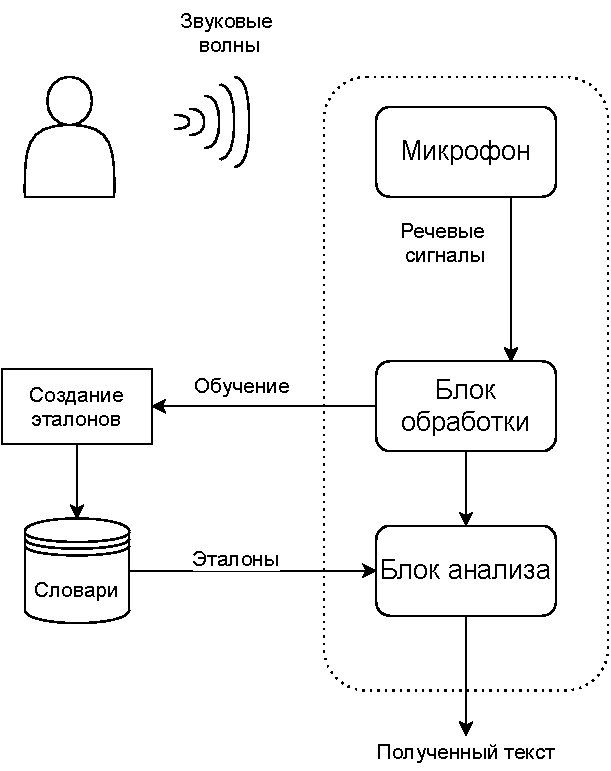
\includegraphics[pages=-, scale=0.9]{./inc/img/3.pdf}
	\caption{Структурная схема системы автоматического распознавания речи}  
	\label{fig:shema}
\end{center}
\end{figure}


Выделение признаков (речевых характеристик) происходит из звукового сигнала, который передается машине. Такой звуковой сигнал, или речевой, так как он передает речь человека, является нестационарным процессом, значения параметров которого непрерывно меняются. Поэтому оценки такого спектра берутся на последовательных кадрах в предположении, что на таких кадрах сигнал является стационарным и характеризуется постоянными фиксированными параметрами. \cite{spektr}


%Системы автоматического распознавания речи широко применяются в медицинских исследованиях, например, когда требуется управлять автономными аппаратами. Важной областью применения систем автоматического распознавания речи является помощью людям с инвалидностью, как для людей с нарушениями речи, так и с проблемами опорно-двигательного аппарата \cite{vvegenie3}.

\textbf{Цель данной научно-исследовательской работы} -- провести обзор методов извлечения речевых характеристик для задачи распознавания речи у людей с дефектами речи.

Для достижения поставленной цели необходимо решить следующие задачи:
\begin{itemize}
	\item рассмотреть классификацию систем автоматического распознавания речи;
	\item рассмотреть возможные дефекты и нарушения речи;
	\item изучить существующие речевые характеристики;
	\item изучить методы извлечения частотных характеристик.
\end{itemize}


